\section{Development}\label{sec:setup}

Throughout, $n\ge3$, indices of vertices and edges lie in $\Zn$, and
$\kappa=(\kappa_i)_{i\in\Zn}$ is a \emph{profile} of prescribed curvatures.
Edge $i$ joins vertex $i$ to vertex $i+1$; it has length $\ell_i=2h_i$, and
$h_i$ is its \emph{half-length}. For $X,Y,W\in\C$ we write
$[X,Y,W]=\operatorname{Im}\bigl(\overline{(Y-X)}\,(W-X)\bigr)$ for twice the
signed area of the triangle $XYW$, and
\begin{equation}\label{eq:menger}
  M(X,Y,W)=\frac{2\,[X,Y,W]}{|X-Y|\,|Y-W|\,|W-X|}
\end{equation}
for its signed Menger curvature; $|M|$ is the reciprocal circumradius.
% Lean: Gluck.Discrete.crossR2, Gluck.Discrete.signedMengerR2 (TangentChord.lean)
% Lean: Gluck.Discrete.dist_circumcenterR2_mul,
%       Gluck.Discrete.dist_circumcenterR2_eq_inv_abs_signedMenger (TabachnikovConverse.lean)

\begin{definition}\label{def:development}
Let $\kappa\in\R^n$, and let $D_\kappa$ be the open set of $h\in\R^n$ with
$|\kappa_ih_{i-1}|<1$ and $|\kappa_ih_i|<1$ for all $i$. For $h\in D_\kappa$
the \emph{turning angle} at vertex $i$ is
\begin{equation}\label{eq:turning-law}
  \theta_i=\arcsin(\kappa_ih_{i-1})+\arcsin(\kappa_ih_i).
\end{equation}
The \emph{headings} are $\psi_j=\theta_0+\theta_1+\dots+\theta_j$ for
$j\in\mathbb N$ (indices of $\theta$ read mod $n$), the \emph{developed
vertices} are
\begin{equation}\label{eq:vertices}
  P_0=0,\qquad P_k=\sum_{j=0}^{k-1}\ell_j\,e^{\ii\psi_j}\quad(k\in\mathbb N),
\end{equation}
and the \emph{closure gap} and \emph{total turn} are
\begin{equation}\label{eq:gap-turn}
  \Gap(\kappa,h)=P_n\in\C,
  \qquad
  \Turn(\kappa,h)=\sum_{i\in\Zn}\theta_i\in\R.
\end{equation}
For $\kappa>0$, $h$ is \emph{moderate} if $h_i>0$, $\kappa_ih_{i-1}<1$ and
$\kappa_ih_i<1$ for all $i$.
\end{definition}
% Lean: Gluck.Discrete.turningAngle, Gluck.Discrete.heading, Gluck.Discrete.vertexR2,
%       Gluck.Discrete.closureGap, Gluck.Discrete.turningSum (Defs.lean);
%       the Lean functions take full lengths ell = 2h and K = 0.
% Lean: Gluck.Discrete.ModerateArc, Gluck.Discrete.moderateArc_zero_iff (Defs.lean)
% Lean: Gluck.Discrete.contDiffAt_closureGap_lengths,
%       Gluck.Discrete.contDiffAt_turningSum_lengths (DormantOpening.lean)

Figure~\ref{fig:development} illustrates the definition for positive curvature
and moderate half-lengths.

\begin{figure}[htbp]
\centering
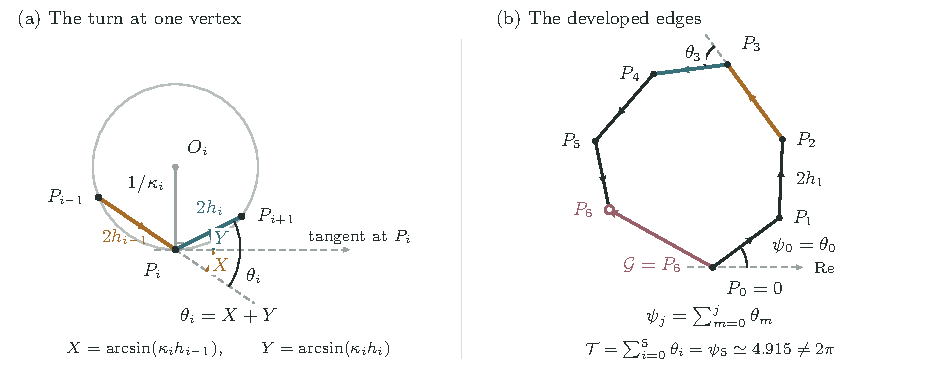
\includegraphics[width=\textwidth]{tabachnikov/figures/development.pdf}
\caption{The quantities in Definition~\ref{def:development}.
(a) The tangent to the circumcircle at $P_i$ splits the exterior turn into
$X$ and $Y$; the incoming edge is continued by a dashed ray.
(b) Edges of length $2h_j$ are placed at headings $\psi_j$.
The highlighted triple $P_2,P_3,P_4$ is the one magnified and rotated in (a),
with $i=3$. The gap arrow runs from $P_0$ to $P_6$; the horizontal reference
shows why the first heading is $\psi_0=\theta_0$.
Here $\Gap\ne0$ and $\Turn\ne2\pi$, so these moderate half-lengths do not
yet give a realization.}
\label{fig:development}
\end{figure}

Both $\Gap$ and $\Turn$ are real-analytic in $(\kappa,h)$ on the open set
where $h\in D_\kappa$, including where some $h_i$ vanish. For moderate $h$
and $\kappa>0$ both arcsines in~\eqref{eq:turning-law} lie in $(0,\pi/2)$, so
$\theta_i\in(0,\pi)$.
% Lean: Gluck.Discrete.turningAngle_pos, Gluck.Discrete.abs_turningAngle_lt_pi (Defs.lean)

\begin{lemma}[Tangent--chord]\label{lem:tangent-chord}
Let $\kappa>0$ and let $h$ be moderate. Then
$M(P_k,P_{k+1},P_{k+2})=\kappa_{k+1}$ for every $k\in\mathbb N$.
\end{lemma}
% Lean: Gluck.Discrete.signedMengerR2_development (TangentChord.lean);
%       Gluck.Discrete.menger_chord_identity (Budget.lean)

\begin{proof}
Put $i=k+1$, $a=\ell_{i-1}$, $b=\ell_i$, $X=\arcsin(\kappa_ia/2)$ and
$Y=\arcsin(\kappa_ib/2)$, so $\theta_i=X+Y$ and $X,Y\in(0,\pi/2)$. The edges
at $P_i$ are $u=ae^{\ii\psi}$ and $w=be^{\ii(\psi+\theta_i)}$ with
$\psi=\psi_{i-1}$. Hence $[P_{i-1},P_i,P_{i+1}]=\operatorname{Im}(\bar
uw)=ab\sin\theta_i$ and, substituting $a=2\sin X/\kappa_i$, $b=2\sin
Y/\kappa_i$,
\[
  \tfrac{\kappa_i^2}{4}|P_{i+1}-P_{i-1}|^2
  =\sin^2\!X+\sin^2\!Y+2\sin X\sin Y\cos(X+Y)=\sin^2(X+Y).
\]
So $\kappa_i|P_{i+1}-P_{i-1}|=2\sin\theta_i$ and
$M=2ab\sin\theta_i/(ab\,|P_{i+1}-P_{i-1}|)=\kappa_i$.
\end{proof}

If $\Gap(\kappa,h)=0$ and $\Turn(\kappa,h)=2\pi$, then $\psi_{j+n}=\psi_j+2\pi$,
so $\ell_{k+n}e^{\ii\psi_{k+n}}=\ell_ke^{\ii\psi_k}$ and, by induction,
$P_{k+n}=P_k$. The development then descends to a closed polygon
$(P_i)_{i\in\Zn}$.
% Lean: Gluck.Discrete.heading_add_n, Gluck.Discrete.vertexR2_add_n,
%       Gluck.Discrete.polygonR2 (Defs.lean)

\begin{definition}\label{def:realization}
Let $\kappa\in\R^n$ be positive. Half-lengths $h$ \emph{realize} $\kappa$ if
$h$ is moderate, $\Gap(\kappa,h)=0$ and $\Turn(\kappa,h)=2\pi$.
\end{definition}
% Lean: Gluck.Discrete.RealizesR2 (Defs.lean); the Lean definition also records
%       IsSimplePolygon, which is automatic by Proposition prop:convex
%       (Gluck.Discrete.isSimplePolygon_of_turningPositive, Convexity.lean).

\begin{proposition}\label{prop:convex}
If $h$ realizes $\kappa$, then $[P_a,P_{a+1},P_c]>0$ whenever
$c\notin\{a,a+1\}$. In particular the polygon $(P_i)_{i\in\Zn}$ is simple and
strictly convex.
\end{proposition}
% Lean: Gluck.Discrete.crossR2_polygonR2_edge_vertex_pos,
%       Gluck.Discrete.support_left_pos, Gluck.Discrete.im_rot_vertex_sub,
%       Gluck.Discrete.isSimplePolygon_of_turningPositive (Convexity.lean)

\begin{proof}
Since every $\theta_i>0$ and $\psi_{j+n}=\psi_j+2\pi$, we have
$\psi_k<\psi_m<\psi_k+2\pi$ for $k<m<k+n$. Fix $k$. For $k\le j$,
\begin{equation}\label{eq:support}
  \operatorname{Im}\bigl(e^{-\ii\psi_k}(P_j-P_k)\bigr)
  =\sum_{m=k}^{j-1}\ell_m\sin(\psi_m-\psi_k),
\end{equation}
and the full sum over $k\le m<k+n$ vanishes. Let $k+1<j<k+n$. If
$\psi_{j-1}-\psi_k\le\pi$, every term in~\eqref{eq:support} is $\ge0$ and the
term $m=k+1$ is $\ell_{k+1}\sin\theta_{k+1}>0$. Otherwise
$\psi_m-\psi_k\in(\pi,2\pi)$ for $j\le m<k+n$, and~\eqref{eq:support} equals
$-\sum_{m=j}^{k+n-1}\ell_m\sin(\psi_m-\psi_k)>0$. Either way
$[P_k,P_{k+1},P_j]>0$. So every vertex off an edge lies in the open left
half-plane of that edge; two non-adjacent edges are separated by the line of
one of them, and consecutive edges meet only in their common vertex.
\end{proof}

A polygon is \emph{coherent} if for every $i$ the triple
$P_{i-1},P_i,P_{i+1}$ is non-collinear and its circumcenter $O_i$ lies in
the open vertex cone
$\{P_i+s(P_{i-1}-P_i)+t(P_{i+1}-P_i):s,t>0\}$.
% Lean: Gluck.Discrete.vertexCone, Gluck.Discrete.CoherentR2 (LocalRegularity.lean)

\begin{proposition}\label{prop:coherent}
If $h$ realizes $\kappa$, the polygon $(P_i)_{i\in\Zn}$ is coherent.
\end{proposition}
% Lean: Gluck.Discrete.coherent_development_moderate,
%       Gluck.Discrete.circumcenterR2_mem_openCone_of_lt (LocalRegularity.lean)

\begin{proof}
Fix $i$, write $u=P_{i-1}-P_i$, $w=P_{i+1}-P_i$, and let $a,b,X,Y$ be as in
the proof of Lemma~\ref{lem:tangent-chord}. Then $\bar uw=-ab\,e^{\ii\theta_i}$,
so $\delta=\operatorname{Im}(\bar uw)=-ab\sin\theta_i\ne0$ and
$\mathcal{C}=\operatorname{Re}(\bar uw)=-ab\cos\theta_i$. The circumcenter is
$O_i=P_i+su+tw$ with
$s=|w|^2(|u|^2-\mathcal C)/(2\delta^2)$ and
$t=|u|^2(|w|^2-\mathcal C)/(2\delta^2)$: indeed
$\langle su+tw,u\rangle=|u|^2(|u|^2|w|^2-\mathcal C^2)/(2\delta^2)=|u|^2/2$,
and likewise for $w$. So $O_i$ lies in the open cone if and only if
$\mathcal C<\min(|u|^2,|w|^2)$. Now
\[
  a^2-\mathcal C=\tfrac{4}{\kappa_i^2}\sin X\bigl(\sin X+\sin Y\cos(X+Y)\bigr)
  =\tfrac{4}{\kappa_i^2}\sin X\sin(X+Y)\cos Y>0,
\]
since $X,Y\in(0,\pi/2)$; the moderate-arc inequalities are used exactly here,
to get $\cos Y>0$. The inequality $b^2-\mathcal C>0$ is symmetric.
\end{proof}

If $\kappa\equiv c>0$, then $h_i=\sin(\pi/n)/c$ realizes $\kappa$: every
$\theta_i=2\pi/n$, and the polygon is the regular $n$-gon.
% Lean: Gluck.Discrete.regularGon_closes (Defs.lean),
%       Gluck.Discrete.realizesR2_const (Convexity.lean)

\subsection{Four-vertex windows and plateau extrema}

\begin{definition}\label{def:dfv}
A profile $\kappa\in\R^n$ has a \emph{strict four-vertex window} at level
$c\in\R$, written $\DFV(\kappa,c)$, if there are integers
$i_1<i_2<i_3<i_4<i_1+n$ satisfying~\eqref{eq:dfv}, indices read mod $n$. A
\emph{plateau maximum run} of $\kappa$ is a cyclic interval
$I=\{a,\dots,a+k\}$ with $k<n-1$ on which $\kappa$ is constant, such that
$\kappa_{a-1}<\kappa_a>\kappa_{a+k+1}$; plateau minimum runs are defined
with the inequalities reversed.
\end{definition}
% Lean: Gluck.Discrete.DFV, Gluck.Discrete.DiscreteFourVertexPos (Converse.lean)
% Lean: Gluck.Discrete.DFV.four_le_period (ConstantRunDFV.lean),
%       Gluck.Discrete.DFV.pos_of_pos (TabachnikovReduction.lean)
% Lean: Gluck.Discrete.PlateauMaxRun, Gluck.Discrete.PlateauMinRun,
%       Gluck.Discrete.IsPlateauLocalMax, Gluck.Discrete.IsPlateauLocalMin
%       (LocalRegularity.lean);
%       Gluck.Discrete.HasTwoPlateauMaxRuns, Gluck.Discrete.HasTwoPlateauMinRuns
%       (TabachnikovReduction.lean)

A window forces $n\ge4$ and, for $\kappa>0$, $c>0$. The runs are the
plateau extrema of Section~\ref{sec:intro}: the strict drops at both ends
force maximality.

\begin{lemma}\label{lem:dfv-plateau}
For $\kappa\in\R^n$ the following are equivalent:
\textup{(a)} $\DFV(\kappa,c)$ for some $c$;
\textup{(b)} $\kappa$ has two disjoint plateau maximum runs;
\textup{(c)} $\kappa$ has two disjoint plateau minimum runs.
\end{lemma}
% Lean: Gluck.Discrete.DFV.plateau_extrema (Converse.lean),
%       Gluck.Discrete.dfv_plateau_extrema (LocalRegularity.lean),
%       Gluck.Discrete.exists_dfv_of_two_plateauMaxRun,
%       Gluck.Discrete.hasTwoPlateauMaxRuns_iff_hasTwoPlateauMinRuns,
%       Gluck.Discrete.discreteFourVertexPos_iff_extrema (TabachnikovReduction.lean)

\begin{proof}
(a)$\Rightarrow$(b),(c). On the integer interval $[i_4-n,i_2]$ the endpoints
are $<c<\kappa_{i_1}$, so a maximum of $\kappa$ on it is attained at an
interior point, and the maximal run of equal values through that point lies
strictly inside the interval. This is a plateau maximum run in
$(i_4-n,i_2)$. The interval $[i_2,i_4]$ gives a disjoint one in
$(i_2,i_4)$. The minimum runs come from $[i_1,i_3]$ and $[i_3,i_1+n]$.

(b)$\Rightarrow$(a). Let $I_1=\{a,\dots,a+k\}$ and $I_2$ be disjoint
plateau maximum runs with values $v_1\le v_2$, and let $a+j$, $0\le j<n$, be
the initial point of $I_2$. Then $j>k$, and $j\ne k+1$, $j\ne n-1$, since
otherwise a strict drop at an end of $I_1$ would give $v_2<v_1$. For $c$
strictly between $\max(\kappa_{a-1},\kappa_{a+k+1})$ and $v_1$, the indices
$a<a+k+1<a+j<a+n-1$ form a window. Apply this to $-\kappa$ for (c).
\end{proof}

Inversion $r\mapsto1/r$ exchanges plateau maxima and minima. So the
hypothesis of Theorem~\ref{thm:main} says exactly that $\kappa=1/r$ has a
strict four-vertex window at some level $c>0$.
% Lean: Gluck.Discrete.discreteFourVertexExtrema_inv (TabachnikovConverse.lean),
%       Gluck.Discrete.tabachnikovProblem2_iff_extrema_form (TabachnikovReduction.lean)

\begin{theorem}\label{thm:dfv-realizes}
Every positive profile with a strict four-vertex window has a realization.
\end{theorem}
% Lean: Gluck.Discrete.realizesR2_of_dfv_fourActive (TabachnikovFourActive.lean);
%       with Proposition prop:regular-polygon:
%       Gluck.Discrete.TabachnikovProblem2 (TabachnikovReduction.lean),
%       Gluck.Discrete.tabachnikovProblem2_all (TabachnikovFourActive.lean)

Theorem~\ref{thm:dfv-realizes} is proved in
Sections~\ref{sec:anchor}--\ref{sec:constructions}.

\begin{proof}[Proof of Theorem~\ref{thm:main}]
Let $\kappa=1/r$ and let $h$ be a realization from
Theorem~\ref{thm:dfv-realizes}, with closed polygon $P$. The polygon is
simple and strictly convex by Proposition~\ref{prop:convex}, and coherent by
Proposition~\ref{prop:coherent}. Lemma~\ref{lem:tangent-chord} and periodicity
give $M(P_{i-1},P_i,P_{i+1})=\kappa_i$, hence the prescribed circumradii.
For the stated local non-concyclicity consequence, if
$P_{i-1},P_i,P_{i+1},P_{i+2}$ lie on a circle with center $O$, then $O$ is the
circumcenter of both non-collinear triples
$P_{i-1},P_i,P_{i+1}$ and $P_i,P_{i+1},P_{i+2}$, so $r_i=|OP_i|=r_{i+1}$.
\end{proof}
% Lean: Gluck.Discrete.tabachnikov_converse_geometric,
%       Gluck.Discrete.signedMengerR2_polygonR2,
%       Gluck.Discrete.eq_circumcenterR2_of_equidist,
%       Gluck.Discrete.vertexCircumradius_eq_of_concyclic (TabachnikovConverse.lean)
